\documentclass[a4paper,12pt]{article}

% Packages
\usepackage{tikz}
\usepackage[utf8]{inputenc} % To use UTF-8 encoding
\usepackage{amsmath} % For advanced math typesetting
\usepackage{graphicx} % To include images
\usepackage{hyperref} % To create hyperlinks
\usepackage{geometry} % To set document margins
\usepackage{comment} % To include comments
\geometry{margin=1in} % 1 inch margins all around
\usetikzlibrary{shapes, arrows.meta}

% Title, Author, and Date
\title{IMDb queueing system analysis}
\author{Michele Lotto and Daniel Jader Pellattiero}
\date{\today}

\begin{document}

\maketitle

\begin{abstract}
Analyse the IMDb replica system performance: identify the bottleneck, measure the maximum system throughput and the optimal number of users.
\end{abstract}

\section{Queueing network model}

\subsection{Network graph}

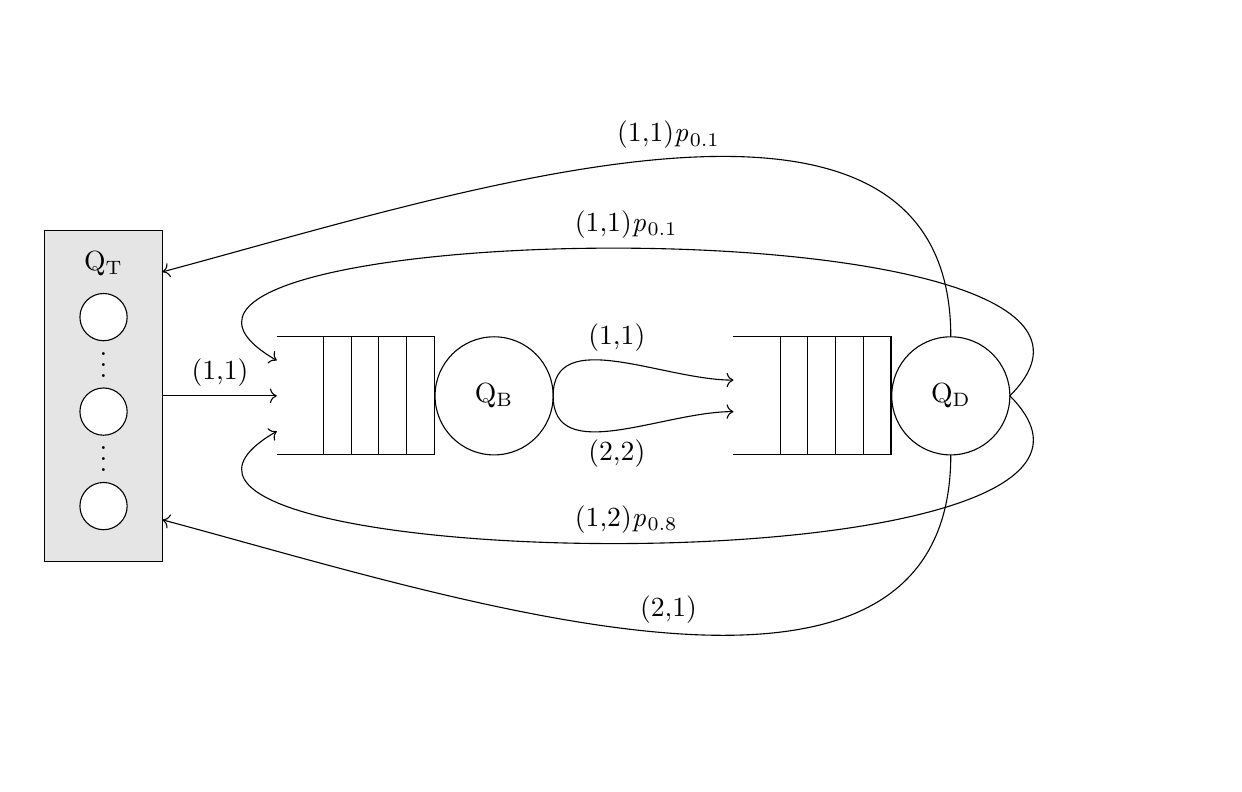
\begin{tikzpicture}
	% Styles
	\tikzstyle{thinking_station} = [rectangle, draw, minimum height=4.2cm, minimum width=1.5cm, fill=gray!20, align=left]
	\tikzstyle{circle_node} = [circle, draw, fill=white, minimum size=6mm, inner sep=0pt]
	\tikzstyle{queue} = [circle, draw, minimum size=1cm, text centered, inner sep=0pt]

	% Thinking station
	\node (QT) [thinking_station] at (0,0) {};
	\node at (0,1.68) {Q\textsubscript{T}};
	% Users belonging to the closed loop
	\node[circle_node] at (0, 1) {};
	\node at (0, 0.5) {$\vdots$};
	\node[circle_node] at (0, -0.2) {};
	\node at (0, -0.7) {$\vdots$};
	\node[circle_node] at (0, -1.4) {};

	% Backend station
	% Queue
	\draw (2.2,0.75) -- ++(2cm,0) -- ++(0,-1.5cm) -- ++(-2cm,0);
	\foreach \i in {1,...,4}
	\draw (4.2cm-\i*10pt,0.75) -- +(0,-1.5cm);
	% Service room
	\draw (4.96,-0.00cm) circle [radius=0.75cm];
	% Label service time
	\node at (4.96,-0.00cm) {Q\textsubscript{B}};

	% Database station
	% Queue
	\draw (8.0,0.75) -- ++(2cm,0) -- ++(0,-1.5cm) -- ++(-2cm,0);
	\foreach \i in {1,...,4}
	\draw (10cm-\i*10pt,0.75) -- +(0,-1.5cm);
	% Service room
	\draw (10.760,-0.00cm) circle [radius=0.75cm];
	% Label service time
	\node at (10.760,-0.00cm) {Q\textsubscript{D}};

	\draw[->]	(QT) to[out=0,in=180] node[above]	{(1,1)} (2.2,0);
	\draw[->]	(5.71,0) to[out=90,in=180] node[above]	{(1,1)} (8.0,0.20);
	\draw[->]	(5.71,0) to[out=-90,in=180] node[below]	{(2,2)} (8.0,-0.20);
	\draw[->]	(11.51,0) to[out=45,in=150] node[above]	{(1,1)\textit{p}\textsubscript{0.1}} (2.2,0.45);
	\draw[->]	(11.51,0) to[out=-45,in=-150] node[above]	{(1,2)\textit{p}\textsubscript{0.8}} (2.2,-0.45);
	\draw[->]	(10.760,-0.75) to[out=-90,in=-15] node[above]	{(2,1)} (0.75,-1.575);
	\draw[->]	(10.760,0.75) to[out=90,in=15] node[above]	{(1,1)\textit{p}\textsubscript{0.1}} (0.75,1.575);
  % (Q1) to[out=90,in=]	node[above]	{\textit{p}\textsubscript{4,5}} (11.0,0);
	
	% (6.760,-0.20cm) to[out=90,in=90] node[above]	{\textit{p}\textsubscript{3,4}} (11.0,0);
\end{tikzpicture}

\subsection{Traffic equations}

\[
\begin{cases}
e_{B1} = e_{T1} + (0.1 \times e_{D1}) \\
e_{B2} = 0.8 \times e_{D1} \\
e_{D1} = e_{B1} \\
e_{D2} = e_{B2} \\
e_{T1} = e_{D2} + (0.1 \times e_{D1}) \\
e_{T1} = 1 \\
\end{cases}
\]

\section{Bottleneck identification}

\section{Miscellaneous}

\begin{itemize}
	\item 
\end{itemize}

\end{document}
